\section{Experimental procedure}
\subsection{Making of the Kinesin-1-stepping assay}
% TODO: describe making of the specimen; create graphic that visualises the purpose of the used chemicals

\subsection{Stream acquisition}
        First the experimental supervisor placed the flow cell holder on the microscope stage. We used an oil objective which has to touch the bottom of the flow cell. The objective has a magnification of 100x and a numerical aperture of 1,46.  
        After the assay was fixed we used a Software called MetaMorph. We chose the camera button. We used a digital Camera by Andor which took greyscaled pictures. Its resolution is $\unit[2.6]{MPixel}$ with 512x512 pixels. The size of one pixel ist $\unit[256]{\mu m^2}$.
        According to the meta data of the movies and pictures the chosen additional magnification of the camera is 1.0x. This means, the pixel size is the original pixel size of the camera. If it would be 2.5x, we could se 2.5 times less, so a pixel would be $A = \unit[256]{\mu m^2} / 2.5 = 102.4$. 
        So we took the TRITC filter and the lamp on the taskbar and watched the live images token by the camera. We searched and focused a cutout where we could see enough MTs. 
        Unfortunately our assay showed that no MT's were fixed in it, so we could not take any pictures. Maybe this was caused by a too thin microtubules solution. This is why we can not compare two different conditions. We used the assay of our co-workers instead. 
        After we focused the MTs, we stop live imaging and take a picture of the MTs which luminescate by rhodamine. \\
        After that we take the GFP filter and choose the laser illumination. Then we choose again live imaging ("show live"). The the TIRF angle will be adjusted.  %note: can we make out the transiotion to the tirf mode?
        Again we choose the TRITC filter on the taskbar, the lamp illumination and take live imaging. We move to a new field of view, focus properly and take an image of the MTs such as in figure \ref{exp:mts}.\\
        \begin{center}
             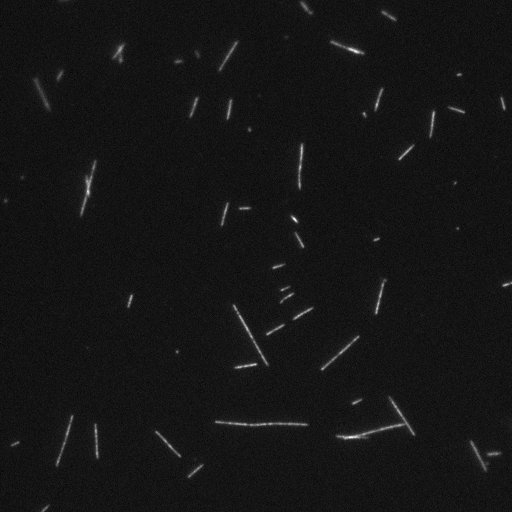
\includegraphics[scale=0.4]{pic/exampleMT.jpeg}  
             \captionof{figure}{Example of an image, where we focused on the MTs}
             \label{exp:mts}
        \end{center}
        Then we save an image of this position. We now switched again to the GFP filter, selected the laser as light source and take live imaging. We can see moving motors. We stop live imaging and take a movie via the acquire button. The number of frames we took is 1000. 
        For one frame the camera needs $\unit[150]{ms}$, so at the end one we wait 150s per video stream. We took 8 movies. 
        When all streams are collected, one can do the data processing with FIESTA. There you can mark the possible trajectories of the motor proteins (as seen in figure \ref{exp:markex1}) and the software will calculate pieces of the picture where the height is the time dimension and the width is the movement. If there is motion, one can mark up the lines and get the time which was needed for the marked distance (see figure \ref{exp:markex2}).
        \begin{center}
                \begin{tabular}{p{7cm}p{5cm}c}
                   \minipanf 
                        \includegraphics[scale=0.05]{pic/example_marked_tubules.jpg}
                        \captionof{figure}{first step marking of the microtubules}
                        \label{exp:markex1}
                   \minipend 
                   &
                   \minipanf
                     \begin{center}
                       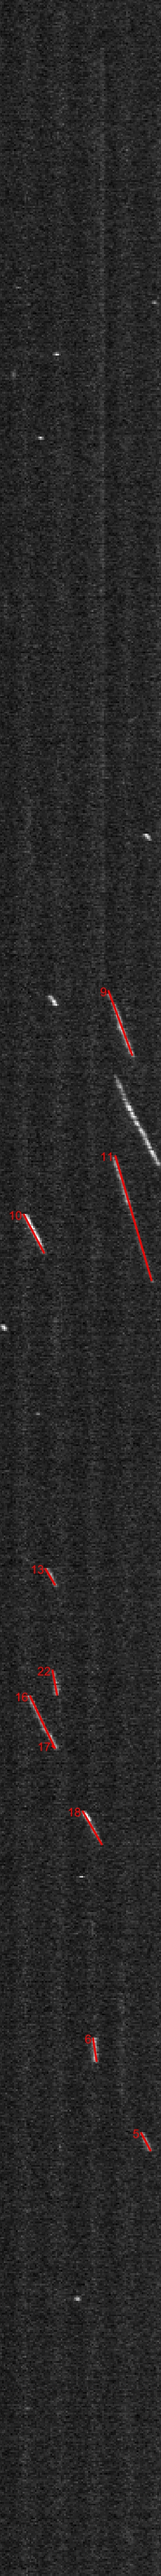
\includegraphics[scale=0.0333]{pic/example_distances_time_marked.jpg}
                       \captionof{figure}{marking of the trajectories of the motor proteins}
                       \label{exp:markex2}
                     \end{center}
                   \minipend
                \end{tabular}    
        \end{center}
